\documentclass{clic_latex_beamer}
\usepackage{tikz}
\usepackage{pgfplots}
\usepackage{pgf-pie}
\usepackage{multicol}

\pgfplotsset{width=7cm,compat=1.10}

\newcommand{\TikZ}{Ti\textit{k}Z}

\begin{document}

\title{Schémas et graphiques en \LaTeX{} avec \TikZ}
\author{David Sandoz}
\date{\today}
\institute{École Polytechnique Fédérale de Lausanne}
\titlegraphic{\ccbysa}

\frame{\titlepage}


\begin{frame}
\frametitle{Table des matières}
\begin{multicols}{2}
\tableofcontents[]
\end{multicols}
\end{frame}

%----------------------
%	Références
%----------------------
 
\begin{frame}
\frametitle{Références}
\begin{itemize}
\item \href{http://paws.wcu.edu/tsfoguel/tikzpgfmanual.pdf }{\emph{\TikZ{} and PGF, Manual for version 1.18}\\ Par Till Tantau (créateur de TikZ)}
\item \href{http://math.et.info.free.fr/TikZ/bdd/TikZ-Impatient.pdf}{\emph{\textbf{\TikZ{} pour l’impatient}}\\ Par Gérard Tisseau et Jacques Duma (en français)}
\item \href{http://pgfplots.sourceforge.net/pgfplots.pdf}{\emph{Manual for Package \uppercase{pgfplots}}\\ Par Dr. Christian Feuersänger}
\item \href{http://pgf-pie.googlecode.com/git/release/pgf-pie-0.2/pgf-pie-manual.pdf}{\emph{Drawing Pie Chart by using pgf-pie}\\ Par Yuan Xu}
\end{itemize}
\end{frame}

%----------------------
%	I - Introduction
%----------------------

\section{Introduction}
\subsection{Alternatives}
\begin{frame}
\frametitle{Alternatives}
Quelles sont les différentes possibilités pour intégrer un schéma dans \LaTeX ?
\begin{itemize}
\item Importation avec \texttt{\textbackslash includegraphics\{\}}
\item Génération du schéma avec du code \LaTeX
\end{itemize}
\end{frame}
 
 % ---- Avantages et inconvénients de TikZ ----
\subsection{Ti\protect\textit{k}Z}
\begin{frame}[fragile]
\frametitle{\TikZ}
Avantages
\begin{itemize}
\item Style et format adapté aux documents \LaTeX
\item Les graphiques créés peuvent contenir du texte écrit en \LaTeX
\item Pas de fichiers externes
\end{itemize}
Inconvéninents
\begin{itemize}
\item N'est pas WYSIWYG
\item Peut être lent (\LaTeX n'est pas fait pour les gros calculs)
\end{itemize}
\end{frame}
 
%----------------------------
%	II - Figures simples (chap 1 et 2 de TikZ pour l'impatient)
%----------------------------

\section{Figures simples}
\subsection{L'environnement}
\begin{frame}[fragile]
\frametitle{L'environnement}
\begin{lstlisting}
\usepackage{tikz}

...

\begin{tikzpicture}
...
\end{tikzpicture}

\end{lstlisting}
\end{frame}
 
\subsection{\textbackslash draw}
\begin{frame}[fragile]
\frametitle{Tracer un cercle}
Voici un cercle

\begin{tikzpicture}
	\draw (0,0) circle (1);
\end{tikzpicture}
en guise de premier exemple

\pause

\begin{lstlisting}
Voici un cercle

\begin{tikzpicture}
    \draw (0,0) circle (1);
\end{tikzpicture}
en guise de premier exemple
\end{lstlisting}
\end{frame}
 
\begin{frame}[fragile]
\frametitle{Différents placements}
\begin{multicols}{2}
Voici un cercle


\begin{tikzpicture}
\draw (0,0) circle (1);
\end{tikzpicture}

en guise de premier exemple
\columnbreak

\pause

\begin{lstlisting}
Voici un cercle


\begin{tikzpicture}
    \draw (0,0) circle (1);
\end{tikzpicture}
    
en guise de premier exemple
\end{lstlisting}

\end{multicols}
\end{frame}
 
\begin{frame}[fragile]
\frametitle{Différents placements}
\begin{multicols}{2}
Dans la figure ci-dessous se trouve un cercle
\begin{figure}

\begin{tikzpicture}
\draw (0,0) circle (1);
\end{tikzpicture}
\caption{Un cercle réalisé avec TikZ}
\end{figure}
\columnbreak

\pause

\begin{lstlisting}
Dans la figure ci-dessous se trouve un cercle
\begin{figure}
  
\begin{tikzpicture}
    \draw (0,0) circle (1);
  \end{tikzpicture}
  \caption{Un cercle réalisé avec TikZ}
\end{figure}
\end{lstlisting}
\end{multicols}
\end{frame}

\begin{frame}[fragile]
\frametitle{Coordonnées}
Les schémas sont centrés sur les dessins et non pas sur l'origine du système de coordonnées.
\begin{multicols}{2}

\begin{tikzpicture}
\draw (0,0) circle (1);
\end{tikzpicture}

\begin{lstlisting}

\begin{tikzpicture}
    \draw (0,0) circle (1);
\end{tikzpicture}
\end{lstlisting}

\columnbreak

\pause


\begin{tikzpicture}
	\draw (3,-2) circle (1);
\end{tikzpicture}

\begin{lstlisting}

\begin{tikzpicture}
    \draw (3,-2) circle (1);
\end{tikzpicture}
\end{lstlisting}


\end{multicols}
\end{frame}

\begin{frame}[fragile]
\frametitle{Échelle}

\begin{multicols}{2}

\begin{tikzpicture}
\draw (0,0) circle (1);
\end{tikzpicture}

\begin{lstlisting}

\begin{tikzpicture}
    \draw (0,0) circle (1);
\end{tikzpicture}
\end{lstlisting}

\columnbreak

\pause

\begin{tikzpicture}[scale=2]
	\draw (0,0) circle (1);
\end{tikzpicture}

\begin{lstlisting}
\begin{tikzpicture}[scale=2]
    \draw (0,0) circle (1);
\end{tikzpicture}
\end{lstlisting}


\end{multicols}
\end{frame}

\begin{frame}[fragile]
\frametitle{Tracer un segment}

\begin{tikzpicture}
	\draw (0,0) -- (1,0);
\end{tikzpicture}

\begin{lstlisting}
\draw (0,0) -- (1,0);
\end{lstlisting}

\pause

\begin{tikzpicture}
	\draw [thick, dashed] (0,0) -- (1,0);
\end{tikzpicture}

\begin{lstlisting}
\draw [thick, dashed] (0,0) -- (1,0);
\end{lstlisting}

\begin{tikzpicture}
	\draw [dotted ,->] (0,0) -- (1,0);
\end{tikzpicture}

\begin{lstlisting}
\draw [dotted, ->] (0,0) -- (1,0);
\end{lstlisting}

Voir les références pour plus d'options

\end{frame}

\begin{frame}[fragile]
\frametitle{\texttt{\textbackslash coordinate(nom) at (x,y)}}
Il peut être plus agréable d'avoir des points avec des noms.

\begin{lstlisting}
\coordinate (A) at (2,3);
\coordinate (B) at (5,1);
\draw (A) -- (B);
\end{lstlisting}

\pause

\begin{tikzpicture}
    \coordinate (A) at (2,3);
    \coordinate (B) at (5,1);
	\draw (A) -- (B);
\end{tikzpicture}


\end{frame}

\begin{frame}[fragile]
\frametitle{Tracer un arc de cercle ou un rectangle}

\begin{multicols}{2}
\begin{tikzpicture}
	\draw (0,0) arc (0:90:1);
\end{tikzpicture}

\begin{lstlisting}
\draw (0,0) arc (0:90:1);
\end{lstlisting}

\columnbreak
\pause


\begin{tikzpicture}
	\draw (0,0) rectangle (2,1);
\end{tikzpicture}


\begin{lstlisting}
\draw (0,0) rectangle (1,2);
\end{lstlisting}

\end{multicols}

\end{frame}

\begin{frame}[fragile]
\frametitle{Tracer une grille}

\begin{multicols}{2}
\begin{lstlisting}
\draw (0,0) grid (4,3);
\end{lstlisting}


\begin{tikzpicture}
\draw (0,0) grid (4,3);
\end{tikzpicture}

\columnbreak
\pause

\begin{lstlisting}
\draw [very thin, gray] (0,0) grid[step=0.5] (4,3);
\end{lstlisting}


\begin{tikzpicture}
\draw [very thin, gray] (0,0) grid[step=0.5] (4,3);
\end{tikzpicture}

\end{multicols}

\end{frame}

\begin{frame}[fragile]
\frametitle{Combinaison de dessins}

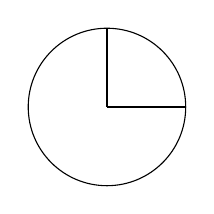
\begin{tikzpicture}
	\draw (0,0) circle (1);
	\draw (0,0) -- (0,1);
	\draw (0,0) -- (1,0);
\end{tikzpicture}


\begin{lstlisting}
\draw (0,0) circle (1);
\draw (0,0) -- (0,1);
\draw (0,0) -- (1,0);
\end{lstlisting}

\end{frame}

\begin{frame}[fragile]
\frametitle{Enchainements de dessins}
\centering

\begin{tikzpicture}
	\draw (0,0) -- (0,1) arc (180:0:1) -- (4,0) rectangle (6,-2) -- (8,-1) circle(1) -- (6,2);
\end{tikzpicture}

\begin{lstlisting}
\draw (0,0) -- (0,1) arc (180:0:1) -- (4,0) rectangle (6,-2) -- (8,-1) circle(1) -- (6,2);
\end{lstlisting}

\end{frame}

\subsection{Ajouter du texte}
\begin{frame}[fragile]
\frametitle{Ajouter du texte}
\centering

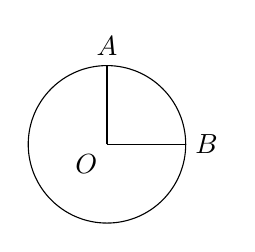
\begin{tikzpicture}
	\draw (0,0) circle (1);
	\draw (0,0) -- (0,1);
	\draw (0,0) -- (1,0);
	\draw (0,0) node[below left]{$O$};
	\draw (0,1) node[above]{$A$};
	\draw (1,0) node[right]{$B$};
\end{tikzpicture}

\pause

\begin{lstlisting}
\draw (0,0) circle (1);
\draw (0,0) -- (0,1);
\draw (0,0) -- (1,0);
\draw (0,0) node[below left]{$O$};
\draw (0,1) node[above]{$A$};
\draw (1,0) node[right]{$B$};
\end{lstlisting}

\end{frame}

\begin{frame}[fragile]
\frametitle{Ajouter du texte}
\centering

\begin{tikzpicture}
	\draw (1,0) arc (0:135:1);
	\draw (0,0) -- (-1.5,1.5);
	\draw (0,0) -- (2,0);
	\draw (0,0) node[below left]{$O$};
	\draw (70:1) node[above right]{$\frac{3\pi}{4}$};
\end{tikzpicture}

\begin{lstlisting}
\draw (1,0) arc (0:135:1);
\draw (0,0) -- (-1.5,1.5);
\draw (0,0) -- (2,0);
\draw (0,0) node[below left]{$O$};
\draw (70:1) node[above right]{$\frac{3\pi}{4}$};
\end{lstlisting} 

\end{frame}
 
%----------------------------
%	III - Graphiques (chap 3 et 5 de TikZ pour l'impatient)
%----------------------------

\section{Graphiques}
\subsection{plot}
\begin{frame}[fragile]
\frametitle{Tracer une courbe linéaire}
$y=\frac{x}{4} \Rightarrow$ Équations paramétriques : $ x=x, y=\frac{x}{4}$

\pause

\begin{lstlisting}
\draw plot (\x, \x/4);
\end{lstlisting}

\pause

\begin{tikzpicture}
	\draw plot (\x, \x/4);
\end{tikzpicture}

\pause

\begin{block}{Par défaut}
 Domaine de -5 à 5.
\end{block}

\end{frame}

\subsection{Domaine}
\begin{frame}[fragile]
\frametitle{Domaine}

\begin{lstlisting}
\draw [domain=-2:2] plot (\x, \x/4);
\end{lstlisting}

\begin{tikzpicture}
	\draw [domain=-2:2] plot (\x, \x/4);
\end{tikzpicture}

\end{frame}

\subsection{Fonctions}
\begin{frame}[fragile]
\frametitle{Fonctions}

Des fonctions standard sont incluses.

\begin{alertblock}{Attention}
 Si des formules contiennent des parenthèses ou des virgules, il faut les écrire entre accolades.\end{alertblock}

\begin{lstlisting}
\draw [domain=-3:1.5] plot (\x, {exp(\x)});
\end{lstlisting}

\begin{tikzpicture}[scale=.5]
\draw [domain=-3:1.5] plot (\x, {exp(\x)});
\end{tikzpicture}

\end{frame}


\begin{frame}[fragile]
\frametitle{Fonctions}

\begin{alertblock}{Attention}
Les fonctions trigonométriques attendent des angles en degrés. Il faut spécifier si l'on souhaite des angles en radiant
\end{alertblock}

\begin{lstlisting}
\draw [domain=-pi:pi] plot (\x, {sin(\x r)});
\end{lstlisting}

\begin{tikzpicture}[scale=1.5]
\draw [domain=-pi:pi] plot (\x, {sin(\x r)});
\end{tikzpicture}

\end{frame}


\begin{frame}[fragile]
\frametitle{Précision}

\begin{block}{Par défaut}
Calcul de 25 points sur la courbe.
\end{block}

\pause

\begin{lstlisting}
\draw [domain=-pi:pi] plot (\x, {sin(5*\x r)});
\end{lstlisting}

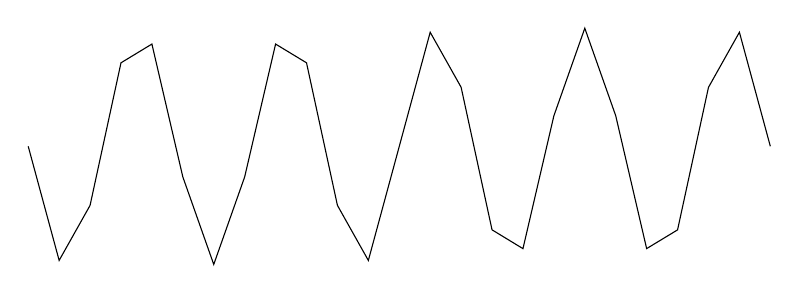
\begin{tikzpicture}[scale=1.5]
\draw [domain=-pi:pi] plot (\x, {sin(5*\x r)});
\end{tikzpicture}

\end{frame}

\begin{frame}[fragile]
\frametitle{Précision}

\begin{lstlisting}
\draw [domain=-pi:pi,samples=200] plot (\x, {sin(5*\x r)});
\end{lstlisting}

\pause

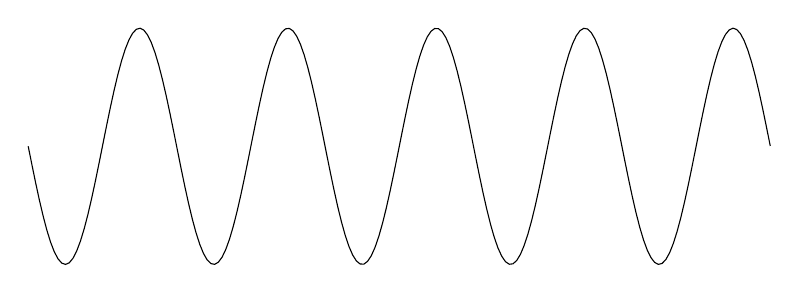
\begin{tikzpicture}[scale=1.5]
\draw [domain=-pi:pi,samples=200] plot (\x, {sin(5*\x r)});
\end{tikzpicture}

\end{frame}

\subsection{Axes et grille}
\begin{frame}[fragile]
\frametitle{Axes et grilles}

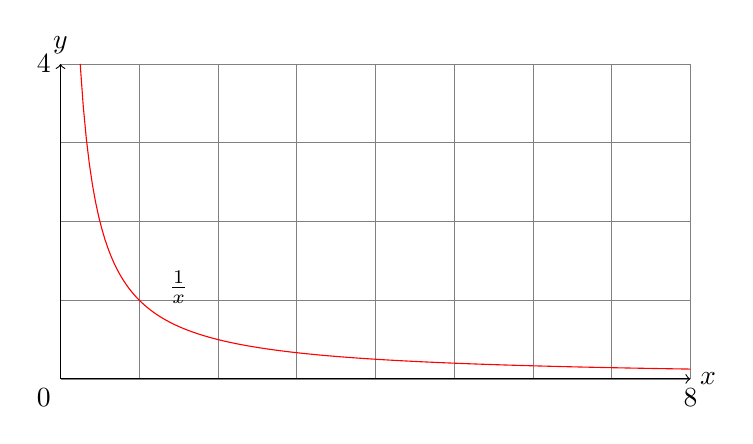
\begin{tikzpicture}
 \draw [very thin, gray] (0,0) grid (8,4);
 \draw [->] (0,0) -- (0,4);
 \draw [->] (0,0) -- (8,0);
 \draw (0,0) node[below left] {0};
 \draw (0,4) node[left] {4};
 \draw (8,0) node[below] {8};
 \draw (0,4) node[above] {$y$};
 \draw (8,0) node[right] {$x$};
 \draw (1.5,1.5) node[below] {$\frac{1}{x}$};
 \draw [domain=0.25:8,samples=200,red] plot (\x, 1/\x);
\end{tikzpicture}

\end{frame}

\begin{frame}[fragile]
\frametitle{Axes et grilles}

\begin{lstlisting}
\draw [very thin, gray] (0,0) grid (8,4);
\draw [->] (0,0) -- (0,4);
\draw [->] (0,0) -- (8,0);
\draw (0,0) node[below left] {0};
\draw (0,4) node[left] {4};
\draw (8,0) node[below] {8};
\draw (0,4) node[above] {$y$};
\draw (8,0) node[right] {$x$};
\draw (1.5,1.5) node[below] {$\frac{1}{x}$};
\draw [domain=0.25:8,samples=200,red] plot (\x, 1/\x);
\end{lstlisting}

Un peu compliqué pour simplement afficher une grille, des axes et les unités ...

\end{frame}

\subsection{PGFPlots}
\begin{frame}[fragile]
\frametitle{PGFPlots}
\begin{itemize}
\item Un package basé sur PGF/\TikZ

\item Simplifie l'insertion de graphiques

\item \begin{lstlisting}
\usepackage{pgfplots}
\end{lstlisting}

\item Toujours entre

\begin{lstlisting}
\begin{tikzpicture}
...
\end{tikzpicture}
\end{lstlisting}
\end{itemize}

\end{frame}

\begin{frame}[fragile]
\frametitle{Exemple de PGFPlots}

\begin{tikzpicture}
\begin{axis}[
   title={$y=\frac{1}{x}$},
   xlabel={$x$},
   ylabel={$y$},
]
   \addplot[
   domain=0.25:8,
   samples=200,
   red,
]
   {1/x};
\end{axis}
\end{tikzpicture}

\end{frame}

\begin{frame}[fragile]
\frametitle{Exemple de PGFPlots}

\begin{lstlisting}
\begin{axis}[title={$y=\frac{1}{x}$}, xlabel={$x$},
             ylabel={$y$}]
   \addplot[domain=0.25:8, samples=200, red]{1/x};
\end{axis}
\end{lstlisting}

\end{frame}


\subsection{Représentation de données}
\begin{frame}[fragile]
\frametitle{Représentation de données}
Peut se faire sans PGFPlots, mais c'est aussi plus facile avec.

\pause

\begin{multicols}{2}
\begin{tikzpicture}[scale=.7]
\begin{loglogaxis}[
    title=Convergence Plot,
    xlabel={Degrees of freedom},
    ylabel={$L_2$ Error},
]
\addplot table {example_data/data_d1.dat};
\end{loglogaxis}
\end{tikzpicture}

\columnbreak

\begin{lstlisting}
\begin{loglogaxis}[
    title=Convergence Plot,
    xlabel={Degrees of freedom},
    ylabel={$L_2$ Error},
]
\addplot table {example_data/data_d1.dat};
\end{loglogaxis}
\end{lstlisting}

\end{multicols}

\end{frame}

\begin{frame}[fragile]
\frametitle{Représentation de données}
\begin{multicols}{2}
\begin{tikzpicture}[scale=.7]
\begin{loglogaxis}[
    title=Convergence Plot,
    xlabel={Degrees of freedom},
    ylabel={$L_2$ Error},
]
\addplot table {example_data/data_d1.dat};
\addplot table {example_data/data_d2.dat};
\addplot table {example_data/data_d3.dat};
\end{loglogaxis}
\end{tikzpicture}

\columnbreak

\begin{lstlisting}
\begin{loglogaxis}[
    title=Convergence Plot,
    xlabel={Degrees of freedom},
    ylabel={$L_2$ Error},
]


\addplot table {example_data/data_d1.dat};
\addplot table {example_data/data_d2.dat};
\addplot table {example_data/data_d3.dat};
\end{loglogaxis}
\end{lstlisting}

\end{multicols}

\end{frame}

\begin{frame}[fragile]
\frametitle{Légende}
\begin{multicols}{2}
\begin{tikzpicture}[scale=.7]
\begin{loglogaxis}[
    title=Convergence Plot,
    xlabel={Degrees of freedom},
    ylabel={$L_2$ Error},
    legend entries={$d=2$,$d=3$,$d=4$},
]
\addplot table {example_data/data_d1.dat};
\addplot table {example_data/data_d2.dat};
\addplot table {example_data/data_d3.dat};
\end{loglogaxis}
\end{tikzpicture}

\columnbreak

\begin{lstlisting}
\begin{loglogaxis}[
    title=Convergence Plot,
    xlabel={Degrees of freedom},
    ylabel={$L_2$ Error},
    legend entries={$d=2$,$d=3$,$d=4$},
]
\addplot table {example_data/data_d1.dat};
\addplot table {example_data/data_d2.dat};
\addplot table {example_data/data_d3.dat};
\end{loglogaxis}
\end{lstlisting}

\end{multicols}

\end{frame}

\begin{frame}[fragile]
\frametitle{Barres d'erreurs}
\begin{multicols}{2}
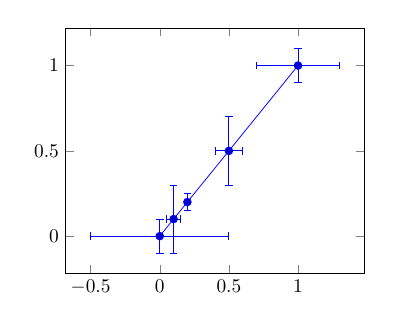
\begin{tikzpicture}[scale=.7]
\begin{axis}
\addplot+[error bars/.cd,
    y dir=both,y explicit,
    x dir=both,x explicit,
]
coordinates {
    (0,0)     +- (0.5,0.1)
    (0.1,0.1) +- (0.05,0.2)
    (0.2,0.2) +- (0,0.05)
    (0.5,0.5) +- (0.1,0.2)
    (1,1)     +- (0.3,0.1)};
\end{axis}
\end{tikzpicture}

\columnbreak

\begin{lstlisting}
\begin{axis}
\addplot+[error bars/.cd,
    y dir=both,y explicit,
    x dir=both,x explicit,
]
coordinates {
    (0,0)     +- (0.5,0.1)
    (0.1,0.1) +- (0.05,0.2)
    (0.2,0.2) +- (0,0.05)
    (0.5,0.5) +- (0.1,0.2)
    (1,1)     +- (0.3,0.1)};
\end{axis}
\end{lstlisting}

\end{multicols}

\end{frame}
\section{Diagrammes}
\subsection{Diagramme en bâtons}
\begin{frame}[fragile]
\frametitle{Diagramme en bâtons}
Toujours avec PGFPlots.
\begin{multicols}{2}

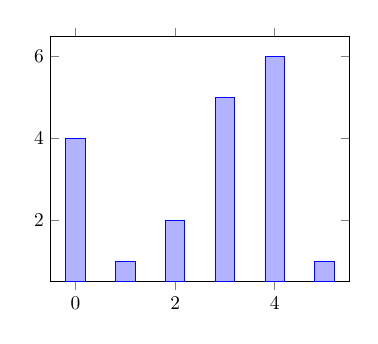
\begin{tikzpicture}[scale=.7]
\begin{axis}[ybar]
\addplot coordinates{(0,4) (1,1) (2,2) (3,5) (4,6) (5,1)};
\end{axis}
\end{tikzpicture}

\columnbreak

\begin{lstlisting}
\begin{axis}[ybar]



\addplot
    coordinates{(0,4) (1,1)
                (2,2) (3,5)
                (4,6) (5,1)};
\end{axis}
\end{lstlisting}

\end{multicols}

\end{frame}


\begin{frame}[fragile]
\frametitle{Diagramme en bâtons}
Toujours avec PGFPlots.
\begin{multicols}{2}

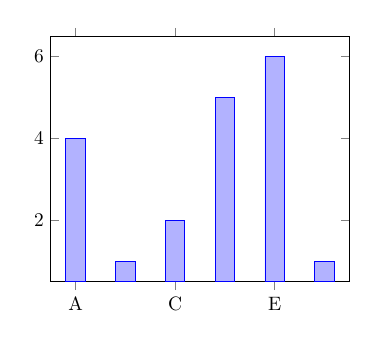
\begin{tikzpicture}[scale=.7]
\begin{axis}[ybar, symbolic x coords={A,B,C,D,E,F}]
\addplot coordinates{(A,4) (B,1) (C,2) (D,5) (E,6) (F,1)};
\end{axis}
\end{tikzpicture}

\columnbreak

\begin{lstlisting}
\begin{axis}[ybar,
    symbolic x coords={A,B,C,D,E,F}]
    
\addplot
    coordinates{(A,4) (B,1)
                (C,2) (D,5)
                (E,6) (F,1)};
\end{axis}
\end{lstlisting}

\end{multicols}

\end{frame}


\begin{frame}[fragile]
\frametitle{Diagramme en bâtons}
Toujours avec PGFPlots.
\begin{multicols}{2}

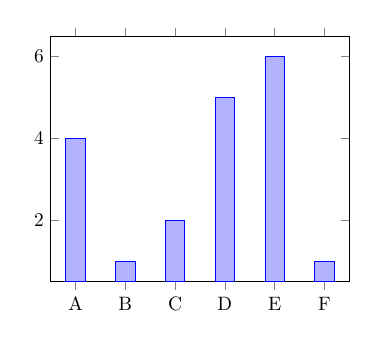
\begin{tikzpicture}[scale=.7]
\begin{axis}[ybar, symbolic x coords={A,B,C,D,E,F}, xtick=data]
\addplot coordinates{(A,4) (B,1) (C,2) (D,5) (E,6) (F,1)};
\end{axis}
\end{tikzpicture}

\columnbreak

\begin{lstlisting}
\begin{axis}[ybar,
    symbolic x coords={A,B,C,D,E,F},
    xtick=data]
\addplot
    coordinates{(A,4) (B,1)
                (C,2) (D,5)
                (E,6) (F,1)};
\end{axis}
\end{lstlisting}

\end{multicols}

\end{frame}

\subsection{Diagramme circulaire}
\begin{frame}[fragile]
\frametitle{Diagramme circulaire}
Avec le package pgf-pie.
\begin{lstlisting}
\usepackage{pgf-pie}
\end{lstlisting}
\end{frame}

\begin{frame}[fragile]
\frametitle{Diagramme circulaire}

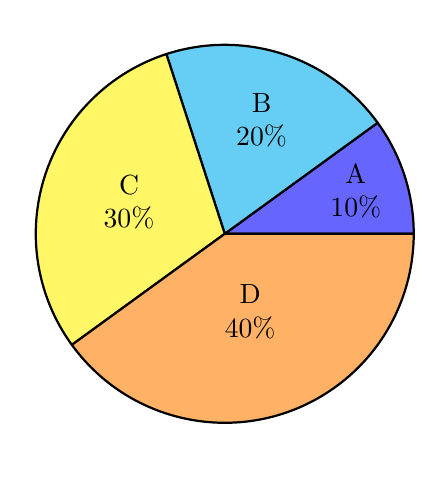
\begin{tikzpicture}[scale=.8]
\pie[text=inside]{10/A, 20/B, 30/C, 40/D}
\end{tikzpicture}


\begin{lstlisting}
\pie[text=inside]{10/A, 20/B, 30/C, 40/D}
\end{lstlisting}

\end{frame}

\begin{frame}[fragile]
\frametitle{Diagramme circulaire}
Pas que circulaire

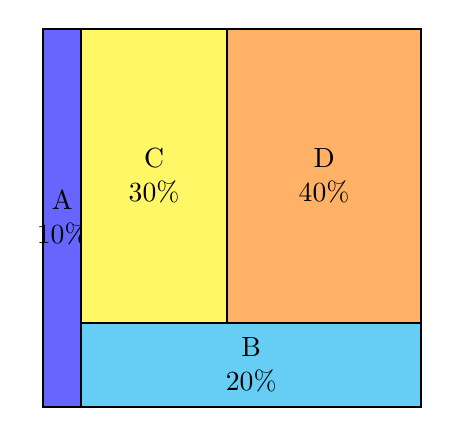
\begin{tikzpicture}[scale=.8]
\pie[square, text=inside]{10/A, 20/B, 30/C, 40/D}
\end{tikzpicture}


\begin{lstlisting}
\pie[square, text=inside]{10/A, 20/B, 30/C, 40/D}
\end{lstlisting}

\end{frame}

\begin{frame}[fragile]
\frametitle{Diagramme circulaire}
Pas que circulaire

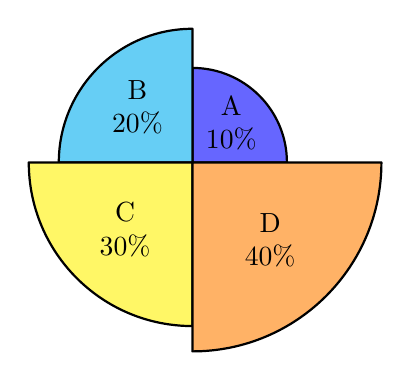
\begin{tikzpicture}[scale=.8]
\pie[polar, text=inside]{10/A, 20/B, 30/C, 40/D}
\end{tikzpicture}


\begin{lstlisting}
\pie[polar, text=inside]{10/A, 20/B, 30/C, 40/D}
\end{lstlisting}

\end{frame}

\begin{frame}[fragile]
\frametitle{Diagramme circulaire}
Pas que circulaire

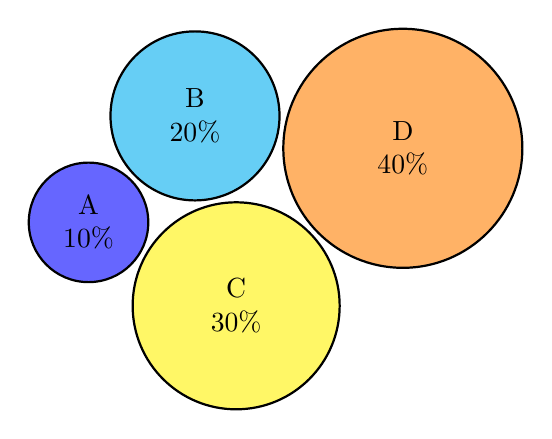
\begin{tikzpicture}[scale=.8]
\pie[cloud, text=inside]{10/A, 20/B, 30/C, 40/D}
\end{tikzpicture}


\begin{lstlisting}
\pie[cloud, text=inside]{10/A, 20/B, 30/C, 40/D}
\end{lstlisting}

\end{frame}


%----------------------------
%	IV - Graphes (chap 6 de TikZ pour l'impatient)
%----------------------------

\section{Graphes}
\begin{frame}[fragile]
\frametitle{Graphes}

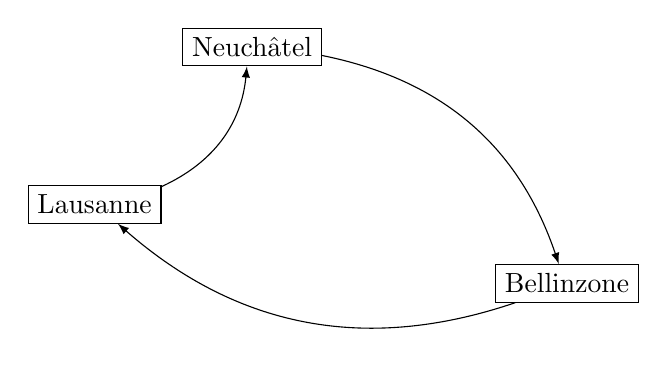
\begin{tikzpicture}
 \node[draw] (L) at (0,0) {Lausanne};
 \node[draw] (B) at (6,-1) {Bellinzone};
 \node[draw] (N) at (2,2) {Neuchâtel};
 \draw[->,>=latex] (L) to[bend right] (N);
 \draw[->,>=latex] (N) to[bend left] (B);
 \draw[->,>=latex] (B) to[bend left] (L);
\end{tikzpicture}

\end{frame}

\subsection{Nœuds}
\begin{frame}[fragile]
\frametitle{Différence entre \texttt{\textbackslash coordinate} et \texttt{\textbackslash node}}

\begin{lstlisting}
\coordinate (L) at (0,0);
\end{lstlisting}

\pause

Un point à utiliser avec \texttt{\textbackslash draw}, mais qui ne s'affiche pas.

\pause
\vspace{1cm}

\begin{lstlisting}
\node[draw] (L) at (0,0) {Lausanne};
\end{lstlisting}

\pause

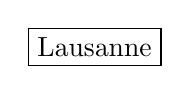
\begin{tikzpicture}
\node[draw] (L) at (0,0) {Lausanne};
\end{tikzpicture}

\end{frame}

\begin{frame}[fragile]
\frametitle{Nœuds}

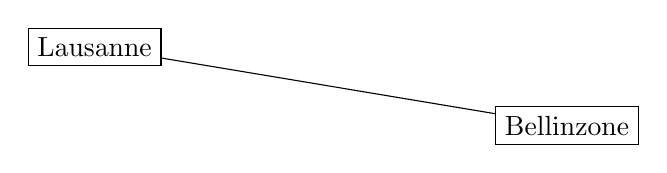
\begin{tikzpicture}
 \node[draw] (L) at (0,0) {Lausanne};
 \node[draw] (B) at (6,-1) {Bellinzone};
 \draw (L) -- (B);
\end{tikzpicture}

\pause

\begin{lstlisting}
\node[draw] (L) at (0,0) {Lausanne};
\node[draw] (B) at (6,-1) {Bellinzone};
\draw (L) -- (B);
\end{lstlisting}

\end{frame}
  
 
%------------------------------------------
%	Exemples et Questions
%------------------------------------------
 

\begin{frame}
\frametitle{Ressources}
De nombreux exemples sur \href{http://www.texample.net/tikz/examples}{texample.net/tikz/examples}
\end{frame}
 
\begin{frame}
\frametitle{Questions ?}
\begin{center}
\Huge Des questions ?
\end{center}
\end{frame}


\end{document}
